
\section{Force and Motion\footnote{
1990-93 Dept. of Physics and Astronomy, Dickinson College. Supported by FIPSE
(U.S. Dept. of Ed.) and NSF. Portions of this material may have been modified
locally and may not have been classroom tested at Dickinson College.
}}

Name \rule{2.0in}{0.1pt}\hfill{}Section \rule{1.0in}{0.1pt}\hfill{}Date \rule{1.0in}{0.1pt}

\textbf{Objectives }

\begin{itemize}
\item To learn how to use a force probe to measure force. 
\item To understand the relationship between forces applied to an object and its motions. 
\item To find mathematical relationships among the force applied to an object, its acceleration, and the directions of the force and acceleration.
\end{itemize}

\textbf{Overview }

In the previous labs, you have used a motion detector to display position-time,
velocity-time and acceleration-time graphs of the motion of different objects.
You were not concerned about how you got the objects to move, i.e., what forces
(pushes or pulls) acted on the objects. From your experiences, you know that
force and motion are related in some way. To start your bicycle moving, you
must apply a force to the pedal. To start up your car, you must step on the
gas pedal to get the engine to apply a force to the road through the tires.

But, exactly how is force related to the quantities you used in the previous
unit to describe motion --- position, velocity and acceleration? In this unit you
will pay attention to forces and how they affect motion. You will apply forces
to a cart, and observe the nature of its resulting motion graphically with a
motion detector.


\textbf{Apparatus} 

\begin{itemize}
\item \textit{Science Workshop 750 Interface}
\item Force probe 
\item Variety of hanging masses 
\item Low friction pulley and string 
\item Motion detector 
\item Dynamics cart (with flag) and track 
\item \textit{DataStudio} software (V, A \& F Graphs application)
\end{itemize}

\textbf{Measuring Forces} 

In this investigation you will use a force probe (also called a force sensor) to measure forces. 
The force probe puts out a voltage signal proportional to the force applied to the arm of the probe. 
Physicists have defined a standard unit of force called the newton, abbreviated N. 
For your work on forces and the motions they cause, it will be more convenient to have the force 
probe read directly in newtons rather than voltage
so the force probe must be calibrated. 
To calibrate the force probe, see \textit{Calibrating Force Sensors} in \textbf{Appendix E: Instrumentation}.

\textbf{Motion and Force} 

Now you can use the force probe to apply measured amounts of force to an object.
You can also use the motion detector, as in the previous units, to examine the
motion of the object. In this way you will be able to establish the relationship
between motion and force.
\vspace{10mm}

\newpage

\textbf{Activity \stepcounter{activity}\arabic{activity}: Pushing and Pulling a Cart} 

In this activity you will move a cart by pushing and pulling it with your hand.
You will measure the force, velocity and acceleration. Then you will be able
to look for relationships between the applied force and the motion quantities.

\begin{enumerate}

\item Calibrate the force probe if you haven't already done so (see \textit{Calibrating Force Sensors} 
in \textbf{Appendix E: Instrumentation}). 
Then set up the cart, force probe and motion detector on the level track as shown in Figure \ref{forcefig1}. 
Measure and record the mass of the cart and force probe assembly (using the compact scale).

\vspace{10mm}

\begin{figure}[hbt]
\begin{center}
{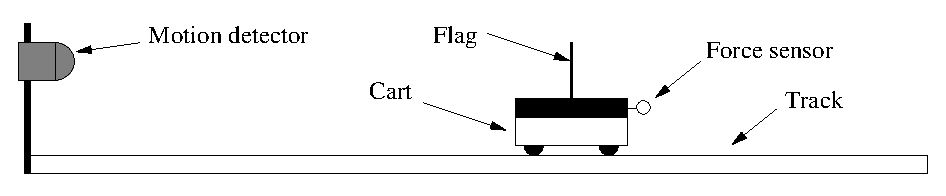
\includegraphics{iqsForce/force1_fig1b.eps}}
\caption{Equipment setup for qualitative measurements of force and motion.}\label{forcefig1}
\end{center}
\end{figure}


\item Suppose you grasp the hook on the force probe and move the cart forwards
and backwards in front of the motion detector. Do you think that either the
velocity or the acceleration graph will look like the force graph? Is either
of these motion quantities related to force? That is to say, if you apply a
changing force to the cart, will the velocity or acceleration change in the
same way as the force?
\vspace{30mm}

\item To test your predictions, open the V, A \& F Graphs application. Grasp the
hook on the force probe and start acquiring data. When you hear the clicks,
pull the cart away from the motion detector, and smoothly stop it. Then push
it back towards the motion detector, and again smoothly stop it. Be sure that
the cart never gets closer than 0.15 m away from the detector and be careful
of the wires. Repeat until you get a good run, and adjust 
the scale of the axes if necessary. Sketch your graphs on the axes below.

\vspace{0.3cm}
\begin{figure}[hbt]
\begin{center}
{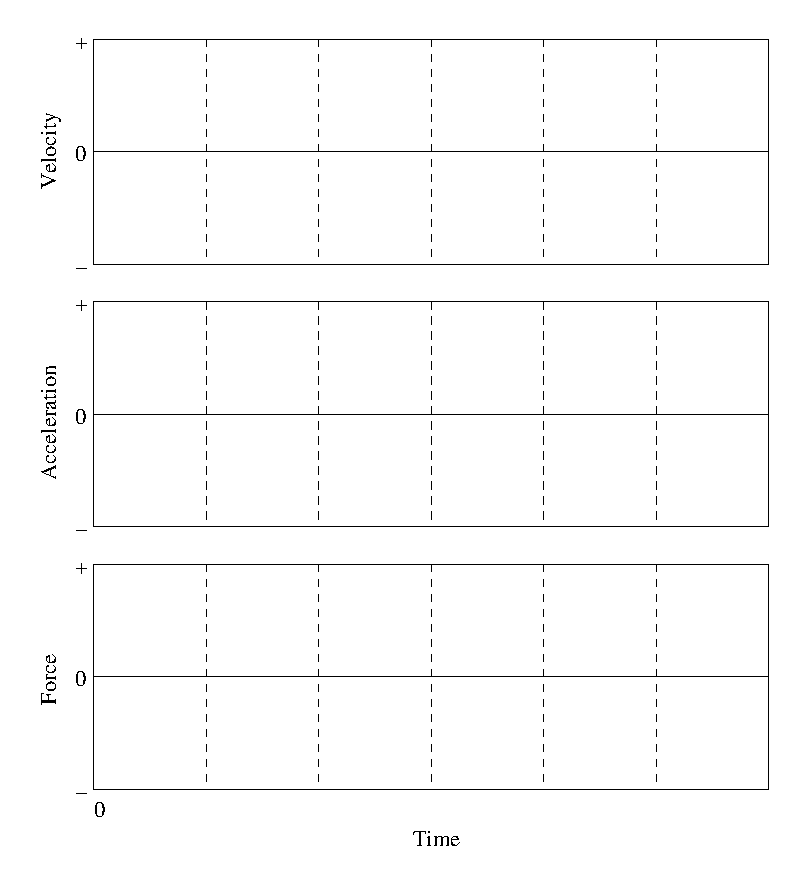
\includegraphics[width=4.4in]{iqsForce/force1_fig2.eps}}
\caption{Velocity, acceleration, and force versus time plots.}
\end{center}
\end{figure}
\vspace{0.3cm}

\item Does either graph--velocity or acceleration--resemble the force graph? Which
one? Explain.
\vspace{20mm}

\item Based on your observations, does it appear that either the velocity or acceleration
of the cart might be related to the applied force? Explain.
\vspace{20mm}

\end{enumerate}

%\newpage

\textbf{Activity \stepcounter{activity}\arabic{activity}: Finding the Relationship Between Acceleration and Force}

\begin{enumerate}

\item Use the {\it SmartTool} in {\it DataStudio} (see {\bf Appendix B: Introduction to DataStudio}) to record twelve or
so sets of acceleration ($a$) and force ($F$) values and enter them in the table below.

\begin{center}
\begin{table}[hbt]
\begin{center}
\begin{tabular}{|c|c|c|c|c|c|}\hline
Trial & $\qquad a(m/s^2)\qquad$ & $\qquad F(N)\qquad$ & Trial & $\qquad a(m/s^2)\qquad$ & $\qquad F(N)\qquad$ \\ \hline
1     &                         &                     & 7     &                         &                     \\ \hline
2     &                         &                     & 8     &                         &                     \\ \hline
3     &                         &                     & 9     &                         &                     \\ \hline
4     &                         &                     & 10    &                         &                     \\ \hline
5     &                         &                     & 11    &                         &                     \\ \hline
6     &                         &                     & 12    &                         &                     \\ \hline
\end{tabular}
\caption{Measured values of force and acceleration.}
\end{center}
\end{table}
\end{center}

\newpage

\item Make a plot of force versus acceleration with properly labeled axes with units.
Attach it to this unit.
Are force and acceleration proportional to each other? Why or why not?

\vspace{15mm}

\item If force is proportional to acceleration, then what is the value of the constant of 
proportionality (Hint: fit your data)?
What are its units? 

\vspace{15mm}

\item What is the equation that relates the force and the acceleration, 

\vspace{15mm}

\item How does the mass of your cart compare with the constant of 
proportionality between force and acceleration?
What does this say about the meaning of the constant of proportionality? About the meaning of mass?

\vspace{15mm}

\item Go around to the other groups in the lab and ask them for their measured values of the
constant of proportionality.
Check that the mass of their cart measured with the scale is similar to yours.
Make a histogram of the results and calculate the average and standard deviation.
For information on making histograms, see \textbf{Appendix C}. For information on calculating the average and
standard deviation, see \textbf{Appendix A}. Record the average and standard deviation here.
Attach the histogram to the unit.

\vspace{15mm}

\item Are the class results for the constant of proportionality consistent with the values from the scale?
Be quantitative in your answer.

\vspace{15mm}

\end{enumerate}

\newpage 

\textbf{Homework} 

\begin{enumerate}

\item A force is applied which makes an object move with the acceleration shown
below. Assuming that friction is negligible, sketch a force-time graph of the
force on the object on the axes below. Explain your answer.

\vspace{1.3cm}
{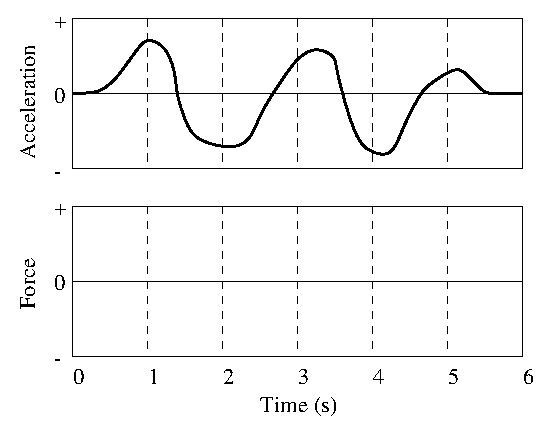
\includegraphics{iqsForce/force1_fig6.eps}}
\vspace{0.3cm}

\item Roughly sketch the velocity-time graph for the object in question 1 on the
axes below, beginning with a $negative$ velocity.

\vspace{0.3cm}
{\par\centering 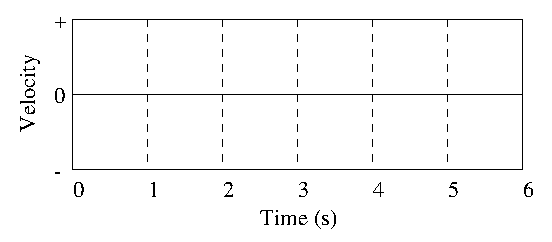
\includegraphics{iqsForce/force1_fig7.eps} \par}
\vspace{0.8cm}

\item A cart can move along a horizontal line (the + position axis). It moves with
the velocity shown below.

\vspace{0.3cm}
{\par\centering 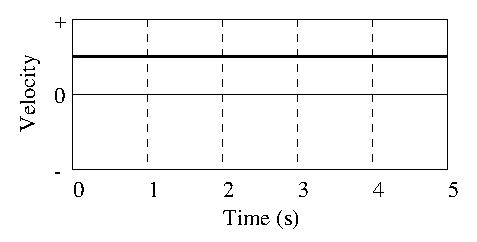
\includegraphics{iqsForce/force1_fig8.eps} \par}
\vspace{0.8cm}

Assuming that friction is so small that it can be neglected, sketch on the axes
that follow the acceleration-time and force-time graphs of the cart's motion.

\vspace{0.3cm}
{\par\centering 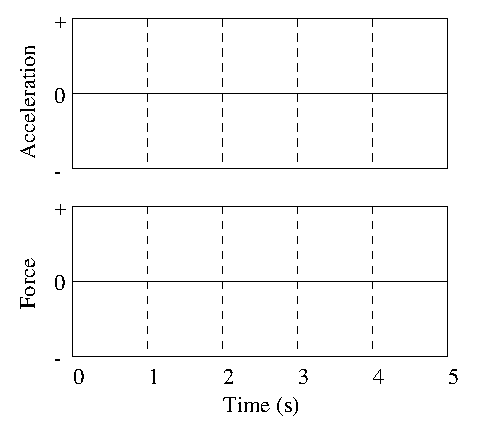
\includegraphics{iqsForce/force1_fig9.eps} \par}
\vspace{0.3cm}

Explain both of your graphs.
\vspace{20mm}

\item The next three questions refer to an object which can move in either direction along a
horizontal line (the + position axis). Assume that friction is so small that
it can be neglected. Sketch the shape of the graph of the force applied to the
object which would produce the motion described. 

The object moves away from the origin with a constant acceleration.

\vspace{0.3cm}
{\par\centering 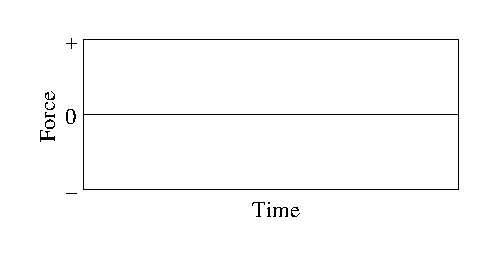
\includegraphics{iqsForce/force1_fig10.eps} \par}
\vspace{0.3cm}

\item The object moves toward the origin with a constant acceleration.

\vspace{0.3cm}
{\par\centering 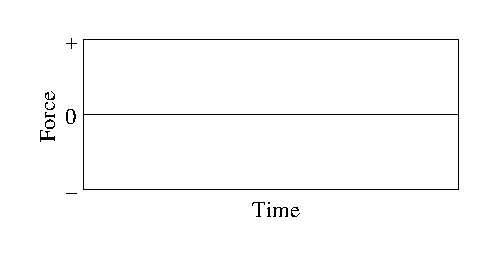
\includegraphics{iqsForce/force1_fig10.eps} \par}
\vspace{0.3cm}

\newpage

\item The object moves away from the origin with a constant velocity.

\vspace{0.3cm}
{\par\centering 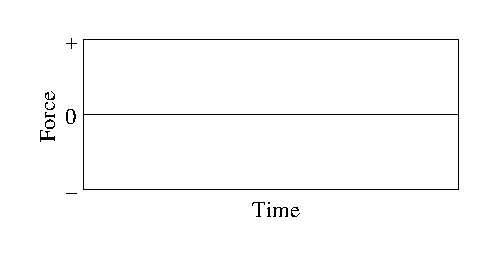
\includegraphics{iqsForce/force1_fig10.eps} \par}
\vspace{0.3cm}

\noindent The next two questions refer to an object which can move along a horizontal line
(the + position axis). Assume that friction is so small that it can be ignored.
The object's velocity-time graph is shown below.

\vspace{0.3cm}
{\par\centering 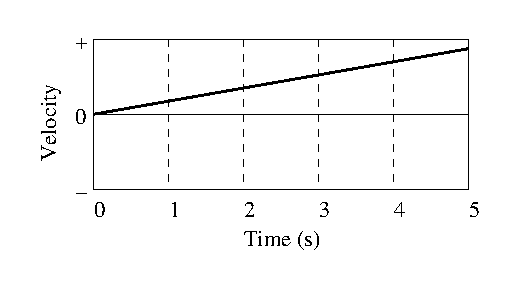
\includegraphics{iqsForce/force1_fig11.eps} \par}
\vspace{0.3cm}

\item Sketch the shapes of the acceleration-time and force-time graphs on the axes
below.

\vspace{0.3cm}
{\par\centering 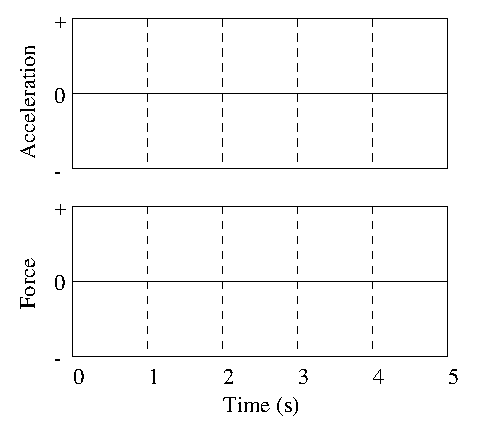
\includegraphics{iqsForce/force1_fig9.eps} \par}
\vspace{0.3cm}

\newpage

\item Suppose that the force applied to the object were twice as large. Sketch
with dashed lines on the same axes above the force, acceleration, and velocity.

The next question refers to an object which can move along a horizontal line (the +
position axis). Assume that friction is so small that it can be ignored. The
object's velocity-time graph is shown below.

\vspace{0.3cm}
{\par\centering 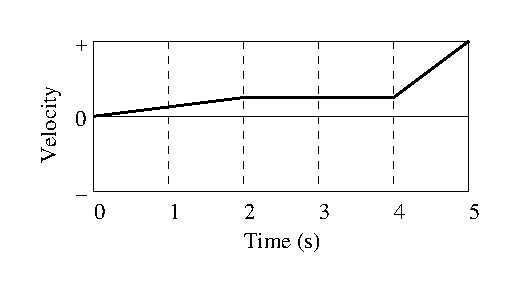
\includegraphics{iqsForce/force1_fig12.eps} \par}
\vspace{0.3cm}

\item Sketch the shapes of the acceleration and force graphs on the axes below.

\vspace{0.3cm}
{\par\centering 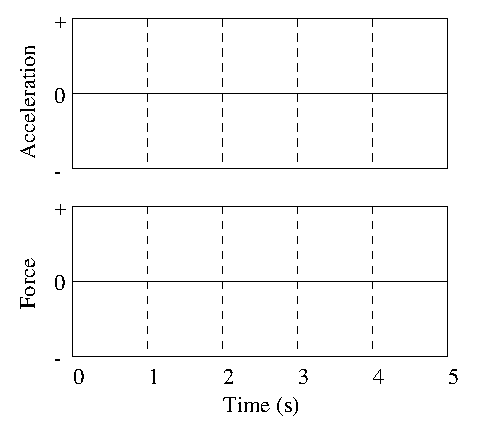
\includegraphics{iqsForce/force1_fig9.eps} \par}
\vspace{0.3cm}

\begin{comment}

The next five questions refer to a toy car which can move in either direction along a
horizontal line (the + position axis).

\vspace{0.3cm}
{\par\centering 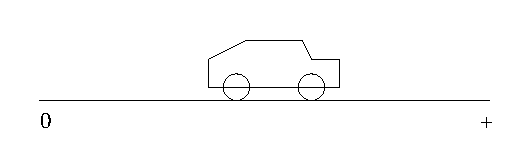
\includegraphics{iqsForce/force2_fig6.eps} \par}
\vspace{0.3cm}

Assume that friction is so small that it can be ignored. Sketch the shape of
the graph of the applied force which would keep the car moving as described
in each statement.

\item The toy car moves away from the origin with a constant velocity.

\vspace{0.3cm}
{\par\centering 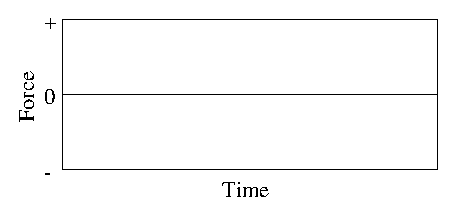
\includegraphics{iqsForce/force2_fig7.eps} \par}
\vspace{0.3cm}

\item The toy car moves away from the origin with a steadily decreasing velocity
(a constant acceleration).

\vspace{0.3cm}
{\par\centering 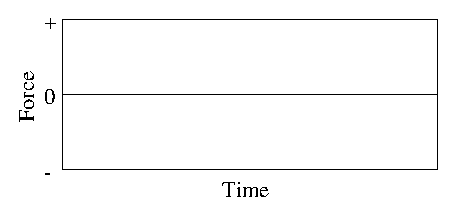
\includegraphics{iqsForce/force2_fig7.eps} \par}
\vspace{0.3cm}

\item The toy car moves away from the origin, speeds up and then slows down.

\vspace{0.3cm}
{\par\centering 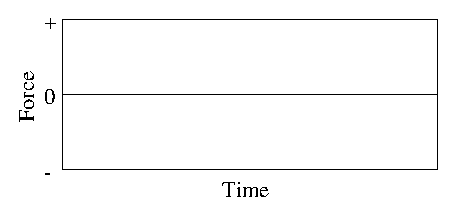
\includegraphics{iqsForce/force2_fig7.eps} \par}
\vspace{0.3cm}

\item The toy car moves toward the origin with a steadily increasing speed ( a
constant acceleration).

\vspace{0.3cm}
{\par\centering 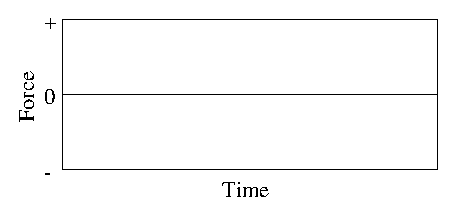
\includegraphics{iqsForce/force2_fig7.eps} \par}
\vspace{0.3cm}

\item The toy car is given a push away form the origin and released. It continues
to move with a constant velocity. sketch the force after the car is released.

\vspace{0.3cm}
{\par\centering 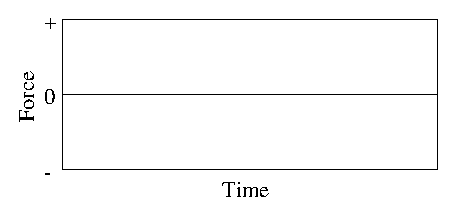
\includegraphics{iqsForce/force2_fig7.eps} \par}
\vspace{1.3cm}

\item A cart is moving toward the right and slowing down, as shown in the diagrams
below. Draw arrows above the cart representing the magnitudes and directions
of the net (combined) forces you think are needed on the cart at $t = 0$ s, 
$t
= 1$ s, etc. to maintain its motion with a steadily decreasing velocity.

\vspace{0.3cm}
{\par\centering 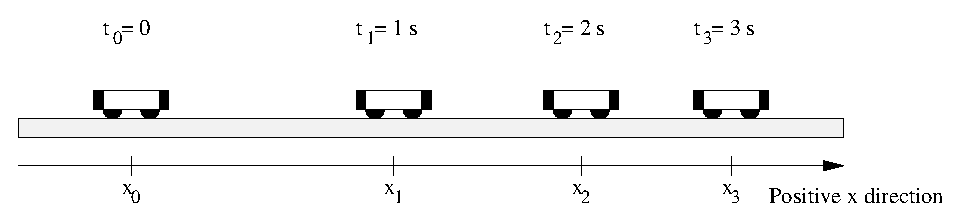
\includegraphics{iqsForce/force2_fig9.eps} \par}
\vspace{0.3cm}

Explain the reasons for your answers.
\vspace{30mm}

\item If the positive direction is toward the right, what is the sign of the force
at $t = 2$ sec in question 9? Explain.
\vspace{30mm}

\end{comment}

\end{enumerate}
